\section{Information Representation and Detection}
\subsection{Sparse Distributed Representation}
The presynaptic input patterns of information that is received by the dendrites, needs to be robust to noise and have a vast encoding capacity, as the neocortex handles an endless stream of sensory input. Empirical evidence shows that the neocortex operates by using sparse representations of information \cite{DBLP:journals/corr/AhmadH16}. In HTM theory, these sparse activation patterns are called \textit{Sparse Distributed Representation}, or SDR. Sparseness is due to the low number of active neurons at any given time, and it is distributed as no information is encoded in a single neuron. The information of the cell activity that the dendrite receives from the presynaptic cells is either active or non-active, and can therefore be modelled as a binary vector \cite{DBLP:journals/corr/AhmadH16}. 


\begin{figure}[ht!]
    \centering
    \resizebox{\textwidth}{!}{\centering
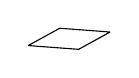
\begin{tikzpicture}
%\draw[help lines] (0,0) grid (10,10); %used just for visualising the positions of objects during construction


\begin{scope}[yshift=-180,yslant=.55,xslant=-1.6,scale=0.4]
        \ColorCells
        \draw (0, 0) grid (\GridSize, \GridSize);
        \coordinate (input);
\end{scope}

\end{tikzpicture}}
    \caption{An example of an SDR, where black squares represent active cells and white squares represent inactive ones. The SDR is represented as matrix for convenience.}
    \label{fig:sdr_ex}
\end{figure}


In \autoref{fig:sdr_ex}, we present an example of presynaptic input, or SDR, represented as a bit vector. Each cell can either be active or inactive, represented as black and white squares respectivly. The entire presynaptic input space of $n$ cells, at time $t$, for a dendritic segment is represented by an $n$-dimensional SDR, $\boldsymbol{X}_t$:


\begin{equation}
    \boldsymbol{X}_t = [b_0,\ b_1,...,\ b_{n-1}]
\end{equation}


\noindent where $b_i \in \mathbb{Z}_2$. The number of active cells is given by $w_X = | \boldsymbol{X}_t |$ and the pattern is considered sparse if $w_X \ll n$. The number of possible encodings the presynaptic input pattern is given by:


\begin{equation}
    \begin{pmatrix} n \\ w_X \end{pmatrix} = \frac{n!}{w_X!(n-w_X)!}
\end{equation}


\subsection{Presynaptic Pattern Detection}
A dendritic segment can also be modelled as a binary vector $\boldsymbol{D}$ of length $n$, which represents both potential and established synaptic connections to the presynaptic input. The active synaptic connections are represented as the non-zero elements, where $b_i$ is the synaptic connection to the presynaptic cell $i$. The number of established connections, represented by $s = | \boldsymbol{D} |$, has been experimentally shown to typically be around 20 to 300 synapses for a dendritic segment. But the potential connections can be in the thousands \cite{DBLP:journals/corr/AhmadH16}. To generate a spike in a dendritic segment, the number of synaptic connections that receive active input form the presynaptic cells needs to exceed a threshold, $\theta$. This threshold can be computed via the dot product of the two binary vectors:

\begin{equation}
    m(\boldsymbol{X}_t,\boldsymbol{D}) \equiv \boldsymbol{X}_t \cdot \boldsymbol{D} \geq \theta
\end{equation}


Where the threshold usually is lower than the number of connections and presynaptic activity, i.e. $\theta \leq s$ and $\theta \leq w_X$. As $\boldsymbol{X}_t$ does not represent the full presynaptic input pattern, but only a subsample, each dendritic segment only learns synaptic connections to some active cells of the entire pattern. How well a dendritic segment detects a pattern is dependent on the value of the NMDA spike threshold, $\theta$, and the robustness to noise in SDR encodings. With lower values of $\theta$ the dendritic branch is able to detect known input patterns easier. However, there is an inherent trade-off in small values of $\theta$, as the dendritic branch are then more likely to detect false positives if there is noise in the input pattern \cite{DBLP:journals/corr/AhmadH16}. 

If $\theta$ is set to a reasonable value, e.g. around 8-20, the probability of false detection due to noise in the SDR will be extremely unlikely. The reason for this is the sheer size of possible combination of ON-bits in the SDR. SDRs corrupted by some noise will not overlap enough to been interpreted as another possible input pattern. Therefore, detection on each dendritic segment with inexact matching has a very low probability of false detection, as described by Ahmad et al. in \cite{DBLP:journals/corr/AhmadH16}.


In each cortical region there are millions of neurons that simultaneously trying to recognise hundreds of patterns. They are able to recognise hundreds of patterns, as there only needs to be between 8 to 20 active synapses to generate an NMDA spike. On each of these neurons there are numerous dendritic branches, that combined have several thousands of synapses on them. Therefore, the robustness of the single dendritic segment needs to be maintained throughout a large neuron network \cite{DBLP:journals/corr/AhmadH16}. 


To quantify the robustness properties in the a larger scale we will first introduce the probability of false positives for an arbitrary number of dendritic segments, of which do not have to belong to the same neuron. Let $M$ be the number of different patterns represented by $M$ different dendritic segments, all of which has the threshold $\theta$ and $s$ number of synapses. The set of the dendritic segments is given by $S = \{ \boldsymbol{D}_0,\ \boldsymbol{D}_1,\ ...,\ \boldsymbol{D}_{M-1}  \}$, where $\boldsymbol{D}_i$ represents a dendritic segment vector. Let $\boldsymbol{X}_t$ be a random presynaptic input, of which is classified as belonging to the set if the following is true:


\begin{equation}
    \boldsymbol{X}_t \in S\ :=\ \exists_{\boldsymbol{D}_i}\ m(\boldsymbol{D}_i, \boldsymbol{X}_t) = True
\end{equation}


There is no false negatives if the number of corrupt bits in $\boldsymbol{X}_t$ is $\leq w_{D_i} - \theta$. The probability of a false positive is given by:

\begin{equation}
    P(\boldsymbol{X}_t \in S) = 1 - (1-P(m(\boldsymbol{X}_t, \boldsymbol{D}_i)))^M
\end{equation}

Which computationally difficult to compute as the probability of individual overlap is extremely unlikely \cite{DBLP:journals/corr/AhmadH16}.

\subsection{The Union Property on Dendritic Segments}
Another important property that comes with the SDR encoding is the ability to group and reliably store a set of SDR with a single SDR representation. This is achieved by taking the union of all the SDRs in a set, and is called the \textit{union property} \cite{DBLP:journals/corr/AhmadH16}. For binary vectors this is equivalent to taking the Boolean OR between all vectors. The ability to store multiple patterns is an important feature of the dendritic segment. In dendritic segments the synapses that respond to different patterns are stored in the same SDR. Thus, multiple presynaptic patterns can cause an NMDA spike to be generated. For a dendritic segment, $\boldsymbol{D}$, to be able to detect an arbitrary number of $M$ synaptic SDRs, we simply take union of all individual synaptic connection vectors, $\boldsymbol{d}_i$:

\begin{equation}
    \boldsymbol{D} = \bigcup_{i=0}^{M-1} \boldsymbol{d}_{i}
\end{equation}


The patterns will be detected as long as $\theta$ number of synapses are active. By increasing the $M$, the number of patterns that a dendritic segment can detect increases, but so does the probability of false detection. Therefore, there is a limit to the amount of ON-bits a dendritic segment can have, before the detection of false positives becomes a problem \cite{DBLP:journals/corr/AhmadH15}. Using unions, we are able to make temporal predictions, temporal pooling, create invariant representations, and create an effective hierarchy \cite{DBLP:journals/corr/AhmadH15}.








\begin{comment}
To prove the robustness to high levels of noise of the SDR encoding, $\boldsymbol{X}$, of $n$ presynaptic cells, we first need to explain the notion of \textit{overlap sets} and then \textit{inexact matching} \cite{DBLP:journals/corr/AhmadH16}. The overlap set allows us to examine the set of vectors of size $n$, that has $a$ ON-bits of which $b$ ON-bits overlap with $\boldsymbol{X}$. The number of vectors that belong to this set is defined as $\Omega_{\boldsymbol{X}}(n,a,b)$. Under the condition that $b \leq |\boldsymbol{X}|$ and $b \leq a$ we can compute the cardinality of this subset of vectors by: 

\begin{equation}
    |\Omega_X(n,a,b)| = \begin{pmatrix} |\boldsymbol{X}| \\ b \end{pmatrix} \times \begin{pmatrix} n - |\boldsymbol{X}| \\ a - b \end{pmatrix}
\end{equation}

\noindent Where the first term represents the number possible subsets of $\boldsymbol{X}$ that share $b$ on-bits, and the second term is all the patterns with $n - |\boldsymbol{X}|$ bits, of which the number of on-bits are $a - b$. Inexact matching allows us to give the probability that a dendritic segment, $\boldsymbol{D}$, will detect a random presynaptic activation pattern, $\boldsymbol{X}_t$  \cite{DBLP:journals/corr/AhmadH16}. The probability is given by the number of possible patterns that the dendritic segment can detect, divided by the number of possible activation patterns.

\begin{equation}
   P(m(\boldsymbol{X}_t, \boldsymbol{D}))  = \frac{\sum^{s}_{b=\theta}|\Omega_{\boldsymbol{D}}(n,w_X,b)|}{\begin{pmatrix} n \\ w_X \end{pmatrix}}
\end{equation}

This gives the probability of a false match for a given dendritic segment \cite{DBLP:journals/corr/AhmadH16}. If the presynaptic input pattern, $\boldsymbol{X}_t$, is corrupted by noise such that $v$ of the on-bits are now off, represented as $\boldsymbol{X}^{\prime}_t$, there is a probability of false negatives. The probability of a false negative increases with $v$, such that $\boldsymbol{X}^{\prime}_t \cdot \boldsymbol{D} < \theta$. As the overlap has to go below the threshold, there is no possibility of a false match if $v$ is sufficiently small, i.e. $v \leq s - \theta$. The computation of the probability of a false negative computed in a similar fashion to false positives \cite{DBLP:journals/corr/AhmadH16}. But instead of we have the cardinality of overlap set of $\boldsymbol{X}^{\prime}_t$ with respect to $\boldsymbol{D}$ in the numerator:

\begin{equation}
    |\Omega_{\boldsymbol{D}}(w_{X^{\prime}},v,b)| = \begin{pmatrix} s \\ b \end{pmatrix} \times \begin{pmatrix} w_{X^{\prime}} - s \\ v - b \end{pmatrix}
\end{equation}

\noindent And thus the probability of a false negative is given by:

\begin{equation}
   P(\boldsymbol{X}^{\prime}_t \cdot \boldsymbol{D} < \theta)  = \frac{\sum^{s}_{b=s - \theta + 1}|\Omega_{\boldsymbol{D}}(w_{X^{\prime}}, v, b)|}{\begin{pmatrix} w_{X^{\prime}} \\ v \end{pmatrix}}
\end{equation}

\end{comment}